\documentclass{standalone}
\usepackage[dvipsnames,svgnames,x11names]{xcolor}
\usepackage{tikz}
\usepackage{pgfplots}
\pgfplotsset{compat = 1.12}
\usepackage{../thesismath}
\begin{document}
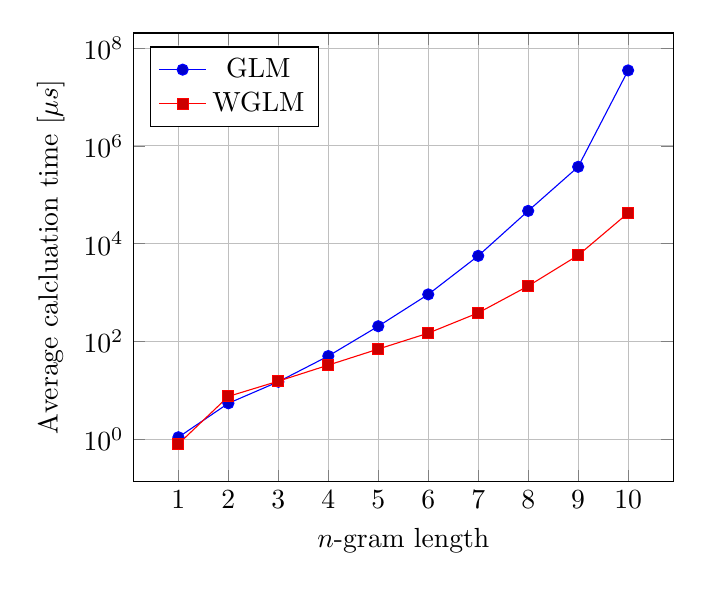
\begin{tikzpicture}[baseline]

\begin{axis}[
  xlabel = {$n$-gram length},
  xtick = {1, ..., 10},
  ylabel = {Average calcluation time [${\mu}s$]},
  ymode = log,
  %yticklabel pos = right,
  minor y tick num = 4,
  grid = major,
  legend entries = {{GLM}, {WGLM}},
  legend pos = north west,
]

% GLM
\addplot table {
  n   us
  % sampled at N = 1000
  1          1.102
  2          5.452
  3         15.045
  4         50.456
  5        205.378
  % sampled at N = 100
  6        920.372
  7       5649.054
  % sampled at N = 1
  8      46971.808
  9     374362.493
  10  35086112.724
};

% WGLM
\addplot table {
  n   us
  % sampled at N = 1000
  1       0.802
  2       7.542
  3      15.461
  4      32.929
  5      70.125
  % sampled at N = 100
  6     148.450
  7     385.515
  8    1364.143
  % sampled at N = 1
  9    5802.023
  10  42471.436
};

\end{axis}

\end{tikzpicture}
\end{document}
